% Constructed and checked from the problem; not a geometric proof.
\documentclass[tikz,border=8pt]{standalone}
\begin{document}
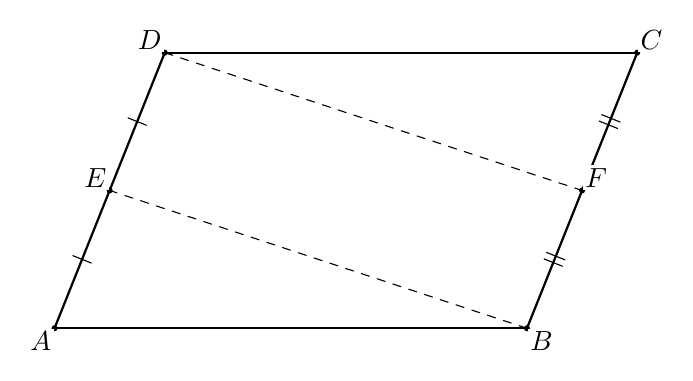
\begin{tikzpicture}[scale=1,line cap=round,line join=round]
\coordinate (p0) at (0,0);
\coordinate (p1) at (6,0);
\coordinate (p2) at (7.4,3.5);
\coordinate (p3) at (1.4,3.5);
\coordinate (p4) at (0.7,1.75);
\coordinate (p5) at (6.7,1.75);
\draw[thick] (p0) -- (p1);
\draw[thick] (p1) -- (p2);
\draw[thick] (p2) -- (p3);
\draw[thick] (p3) -- (p0);
\draw[dashed] (p1) -- (p4);
\draw[dashed] (p3) -- (p5);
\draw (0.2331976,0.9217209) -- (0.4668024,0.8282791);
\draw (0.9331976,2.6717209) -- (1.1668024,2.5782791);
\draw (6.2168453,0.8808401) -- (6.45045,0.7873982);
\draw (6.24955,0.9626018) -- (6.4831547,0.8691599);
\draw (6.9168453,2.6308401) -- (7.15045,2.5373982);
\draw (6.94955,2.7126018) -- (7.1831547,2.6191599);
\fill (p0) circle (1.1pt) node[fill=white,inner sep=1pt,below left] {$A$};
\fill (p1) circle (1.1pt) node[fill=white,inner sep=1pt,below right] {$B$};
\fill (p2) circle (1.1pt) node[fill=white,inner sep=1pt,above right] {$C$};
\fill (p3) circle (1.1pt) node[fill=white,inner sep=1pt,above left] {$D$};
\fill (p4) circle (1.1pt) node[fill=white,inner sep=1pt,above left] {$E$};
\fill (p5) circle (1.1pt) node[fill=white,inner sep=1pt,above right] {$F$};
\end{tikzpicture}
\end{document}
